% v2-acmlarge-sample.tex, dated March 6 2012
% This is a sample file for ACM large trim journals
%
% Compilation using 'acmlarge.cls' - version 1.3, Aptara Inc.
% (c) 2011 Association for Computing Machinery (ACM)
%
% Questions/Suggestions/Feedback should be addressed to => "acmtexsupport@aptaracorp.com".
% Users can also go through the FAQs available on the journal's submission webpage.
%
% Steps to compile: latex, bibtex, latex latex
%
\documentclass[prodmode,acmtap]{acmlarge}

% Metadata Information
\acmVolume{2}
\acmNumber{3}
\acmArticle{1}
\articleSeq{1}
\acmYear{2010}
\acmMonth{5}

% Package to generate and customize Algorithm as per ACM style
\usepackage[ruled]{algorithm2e}
\usepackage{comment}
\usepackage{todonotes}
\usepackage[square,sort]{natbib}
\usepackage{graphics}
\usepackage{caption}
\SetAlFnt{\algofont}
\SetAlCapFnt{\algofont}
\SetAlCapNameFnt{\algofont}
\SetAlCapHSkip{0pt}
\IncMargin{-\parindent}
\renewcommand{\algorithmcfname}{ALGORITHM}

% Page heads
\markboth{A. Sperlea and D. Arneson}{Demonstrating that Epigenomic Modifications are Cell-Type Specific Through Clustering and Identifying Biologically Relevant Domains}

% Title portion
\title{Demonstrating that Epigenomic Modifications are Cell-Type Specific Through Clustering and Identifying Biologically Relevant Domains}
\author{ADRIANA SPERLEA and DOUGLAS ARNESON \affil{University of California Los Angeles}}
% NOTE! Affiliations placed here should be for the institution where the
%       BULK of the research was done. If the author has gone to a new
%       institution, before publication, the (above) affiliation should NOT be changed.
%       The authors 'current' address may be given in the "Author's addresses:" block (below).
%       So for example, Mr. Fogarty, the bulk of the research was done at UIUC, and he is
%       currently affiliated with NASA.

\begin{abstract}
Need to write Abstract Together
\end{abstract}

\terms{Epigenomics}
\keywords{Chromatin modifications, PCA, Clustering, F-Score, Purity}

\acmformat{Adriana Sperlea and Douglas Arneson. 2015. Demonstrating that Epigenomic Modifications are Cell-Type Specific Through Clustering and Identifying Biologically Relevant Domains.}
% At a minimum you need to supply the author names, year and a title.
% IMPORTANT:
% Full first names whenever they are known, surname last, followed by a period.
% In the case of two authors, 'and' is placed between them.
% In the case of three or more authors, the serial comma is used, that is, all author names
% except the last one but including the penultimate author's name are followed by a comma,
% and then 'and' is placed before the final author's name.
% If only first and middle initials are known, then each initial
% is followed by a period and they are separated by a space.
% The remaining information (journal title, volume, article number, date, etc.) is 'auto-generated'.

\begin{document}

\begin{bottomstuff}
STATSM254 Final Report
\end{bottomstuff}


\maketitle

% Head 1
\section{Introduction}

The recent availability of epigenomic data sets such as histone modifications or DNA methylation, coupled with the growing popularity of applying machine learning techniques to genomic data have enabled the computational imputation of genome-wide cross-sample epigenetic marks. In the paper by \citealp{Ernst15}, the authors developed a method called ChromImpute that accurately predicts a variety of epigenomic data in 127 human cell lines originating from a diverse set of tissues.
Previous work has shown that although histone modifications are not cell type specific at promoter and transcription factor binding sites, they show a high level of cell type specificity at enhancer sites, which they are strongly associated with. Thus, it is expected that similar cell types will exhibit similar epigenetic marks. Here, we show that the imputed data from \citealp{Ernst15} preserves the cell-type specific aspect of chromatin modifications by running a principal component analysis (PCA) on the dataset from their paper, and then clustering the resulting distribution of cell lines. Certain histone modifications were more cell type specific and thus more accurately assigned similar types to the same cluster.
We attempted to gain insight into the biological function of the genomic regions that proved to be most important to the PCA in a certain chromatin modification, and particularly to those that were present across marks by cross-checking these regions with known annotations of the human genome. These regions fell predominantly in non-coding regions, but exhibited a potential association with enhancer sites.

% Head 2
\section{Principal Component Analysis}

The imputed data from \citealp{Ernst15}. consists of 9 different chromatin modifications in 127 different cell-types, with a corresponding p-value for each bin of 500 base pairs in the genome indicating the likelihood of having that particular mark at that location. In order for our problem to remain computationally tractable we restricted our analysis to chromosome 21, though data is available for the entire human genome. For each of these 9 chromatin modifications we normalized the data such that the p-values for every location in the genome have mean 0 and variance 1 (Figure ~\ref{fig:figure1}). 

\begin{figure}[tp]
\centering
\begin{minipage}{.5\textwidth}
	\centering
	\scalebox{.45}{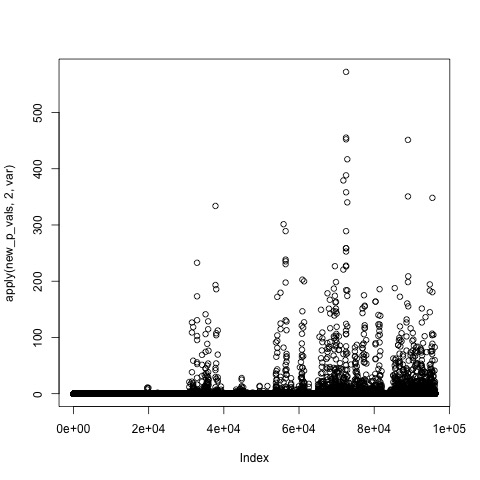
\includegraphics{varPlot1}}
\end{minipage}%
\begin{minipage}{.5\textwidth}
	\centering
	\scalebox{.45}{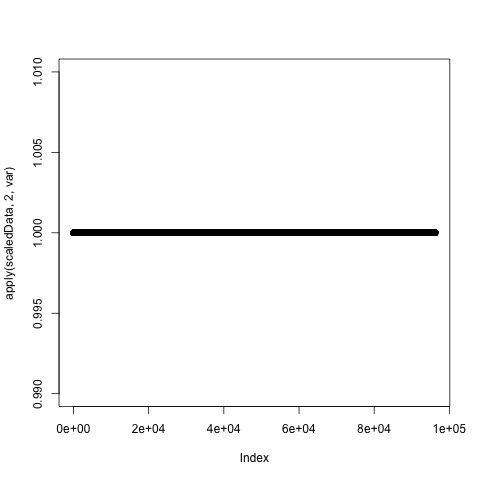
\includegraphics{varPlot2}}	
\end{minipage}	
\captionof{figure}{H3Kme27ac variance of p-values across chromosome 21 before and after normalization. After normalization, the p-values show an uniform distribution. See Supplementary Materials for the variance of the other chromatin modifications before and after normalization.}
\label{fig:figure1}
\end{figure}

After normalization, we ran a principal component analysis on each of the 9 chromatin modifications. Our results show that upwards of 30 principal components were necessary to explain 85\% of the variance which is a common threshold used in the literature, but by analyzing the scree plots of the variance of each component we were able to restrict the number of important components further. We used the broken-stick method \citealp{Cang07} to quantify the point in the turn in the scree graph where retaining an additional principal component would be of no benefit (Figure ~\ref{fig:figure2}). The number of principal components retained in each epigenetic mark are available in Table~\ref{table:tab1}.

% Table
\begin{table}[t]
\tbl{Number of Principal Components Retained in Each Epigenetic Mark}{
\begin{tabular}{|l|l|l|l|l|l|l|l|l|l|}
\hline
Epigenetic Mark                         & DNase & H3K4me1 & H3K4me3 & H3K9ac & H3K9me3 & H3K27ac & H3K27me3 & H3K36me3 & RNAseq \\ \hline
Number of principal components retained & 3     & 5       & 3       & 4      & 5       & 4       & 3        & 5        & 6      \\ \hline
\end{tabular}}
\begin{tabnote}
The number of principal components retained in the analysis of each epigenetic mark.
\end{tabnote}
\label{table:tab1}
\end{table}

\begin{table}[t]
\tbl{F-Scores and Purity Scores}{
\begin{tabular}{|l|l|l|l|l|l|l|l|l|l|}
\hline
        & DNase    & H3K27ac  & H3K27me3  & H3K36me3  & H3K4me1   & H3K4me3   & H3K9ac   & H3K9me3   & RNAseq   \\ \hline
F-Score & 0.52380  & 0.697478 & 0.4895104 & 0.5545454 & 0.5726495 & 0.4171779 & 0.713178 & 0.3972602 & 0.603351 \\ \hline
Purity  & 0.769230 & 1        & 0.777777  & 1         & 1         & 0.8181818 & 1        & 1         & 1        \\ \hline
\end{tabular}}
\begin{tabnote}
Add any caption you'd like here.
\end{tabnote}
\label{table:tab2}
\end{table}

\begin{figure}[tp]
\centering
\scalebox{.45}{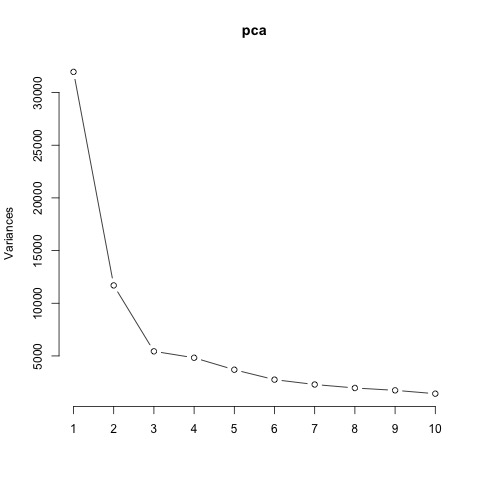
\includegraphics{screePlot}}
\captionof{figure}{Scree plot of the proportion of variance explained by each principal component for the DNase assay. The broken stick method selects 3 principal components, because the eigenvalue of the 4th component is not larger than the value given by the broken-stick distribution.}
\label{fig:figure2}
\end{figure}

\section{Clustering}

Subsequent to data normalization and principal component selection, an exploratory visualization of the transformed data was conducted to determine how best to proceed (Figure 1). This visualization revealed that although some tissue groups were tightly clustered (indicated by red circles), many of the points on the plot were not well clustered, or would intermingle with points from a different tissue group. 



Our initial schema was to leverage a k-means approach to identify clusters within the data (in the number of PC dimensions as determined by the skree plots). This approach was based on the hypothesis that the variance from certain histone modifications would allow classification of different tissues groups in the form of clusters [cite]. To facilitate this procedure, the originally furnished dataset was subset to eliminate particular tissue groups that made the task less feasible. The ENCODE2012 and Other tissue groups had representative cell types across multiple tissue types. These samples would be difficult to reclassify under the appropriate tissue group, and not all fit directly into the already established subcategories. Thus, the samples that comprised these two tissue groups were removed from the collection of data. Although this solution made the data more manageable, further reduction was required.  The objective function of k-means (Equation 1) has the intrinsic property of giving more weight to larger clusters; this property can be seen in Figure 2. To correct for this cluster size bias, smaller tissue groups, those with less than 5 samples per group, were also removed (mesench, neurosph, thymus, and sm. muscle). 

\section{Variance Analysis}
Since similar cell types seemed to cluster together in our analysis, we then sought to understand whether certain genomic regions are more important than others in explaining the similarity of the cell-types, which could point to these regions having an important biological function. However, the weight of each region on the important principal components was at most 0.01 for any genomic region and epigenomic mark. 
Even though the differences in the loadings of the principal components were small, this could be caused by the fact that the data is binned in regions of 500 base pairs which might be either too large or too small to have a significant contribution. Since higher resolution data was not immediately available, we binned the hundred most important regions into segments of 5kb to see whether certain 5kb regions contain more of the important loadings than others. Since certain 5kb regions seemed to be more important than others (Figure ~\ref{fig:figure10}), we investigated whether the regions where the top loadings clustered had a biological function. A preliminary analysis using the UCSC Genome Browser(cite), showed that these fell predominantly in non-coding regions. However, since previous work points to a connection between histone modifications and enhancer sites, which can be far from the coding region they regulate, we overlapped these regions with the enhancer sites predicted by ChromHMM in 9 different cell types. Even though the ChromHMM tracks are imputed, they provide the most comprehensive and widely accepted annotation of human enhancer sites across cell-types. Although some regions overlapped with strong or weak enhancer sites, this overlap was not consistent enough for any further claims to be made.

\begin{figure}[tp]
\centering
\scalebox{.45}{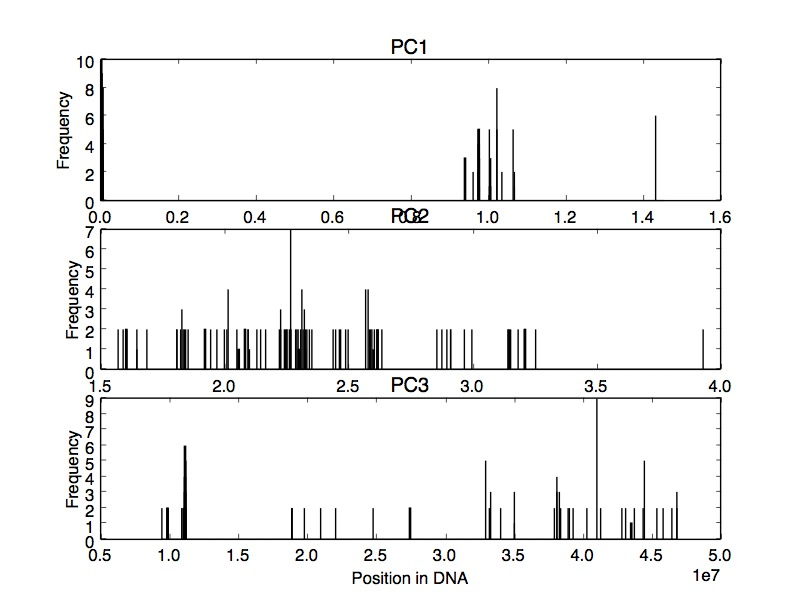
\includegraphics{regions}}
\captionof{figure}{Histogram of the distribution of 500 base pair bins across the genome, binned together into regions of 5kb for the H3K4me3 histone modification. Certain bins show a higher frequency of important regions than others. See Suplementary Ma}
\label{fig:figure10}
\end{figure}

\begin{thebibliography}{}
\bibitem[Ernst and Kellis, 2015]{Ernst15} Jason Ernst and Manolis Kellis. (2015) Large-scale imputation of epigenomic datasets for systematic annotation of diverse human tissues, {\it Nature Biotechnology}, {\bf 33}, 364-376.
\bibitem[Cangelosi and Goriely, 2007]{Cang07} Richard Cangelosi and Alain Goriely. (2007) Component retention in principal component analysis with application to cDNA microarray data, {\it Biology Direct}, {\bf 2}, 2.
\end{thebibliography}
\bibitem[Ernst and Kellis, 2012]{Ernst12} Jason Ernst and Manolis Kellis. (2012) ChromHMM: automating chromatin-state discovery and characterization, {\it Nature Methods}, {\bf 9}, 215-216.

\received{February 2009}{July 2009}{October 2009}


\elecappendix

\end{document}
% End of v2-acmlarge-sample.tex (March 2012) - Gerry Murray, ACM
